\chapter{Discussion}\label{chap:discussion}

In this chapter, we discuss the findings of this thesis presented in Chapter
\ref{chap:results}, which we will summarize in Section \ref{sec:key_findings}.
We then formulate a set of recommendations in Section
\ref{sec:discussion_recommendations}, and then highlight some limitations and
future directions of research in Section \ref{sec:discussion_limitations}.

\section{Key Findings}\label{sec:key_findings}

Overall, we found that \acrshort{mmd} behaved surprisingly well on graphs extracted from
proteins (e.g. see Figure \ref{fig:mmd_consistent_eps}). This finding is
somewhat surprising considering recent findings indicating the relative
instability of \acrshort{mmd} on synthetic graphs such as Watts-Strogatz graphs and
Barabási–Albert graphs under some combinations of kernels and descriptors
\citep{obray2022evaluation}. While we certainly found unstable configurations
(see for instance Figure \ref{fig:mmd_consistent_eps} upper left pane with the degree histogram),
this was not the rule. We hypothesize that this is due to the highly structured
nature of the graphs used in this thesis (see Figure
\ref{fig:er_comparison_8a_graph} for an example).

\begin{figure}
  \centering
  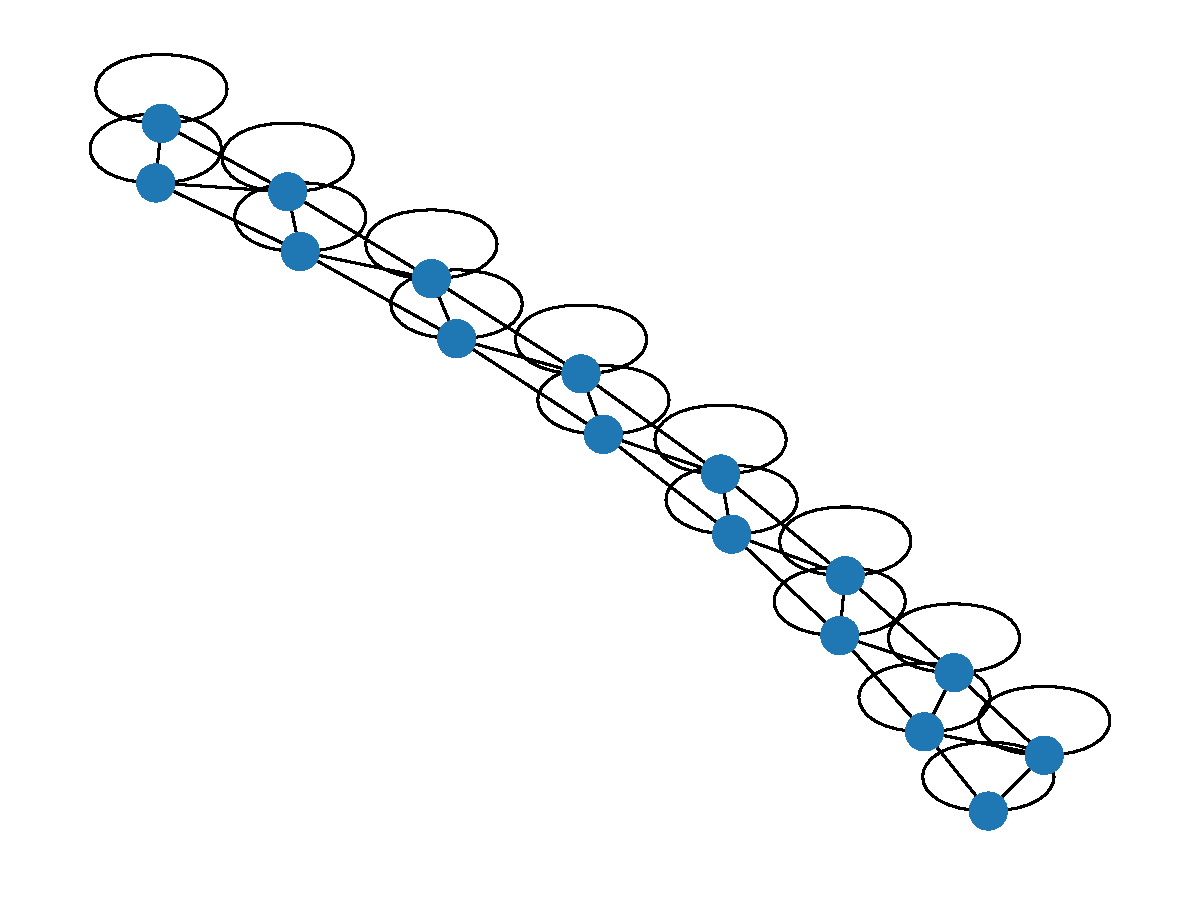
\includegraphics[width=0.4\textwidth]{./figures/results/8_a_graph.pdf}
  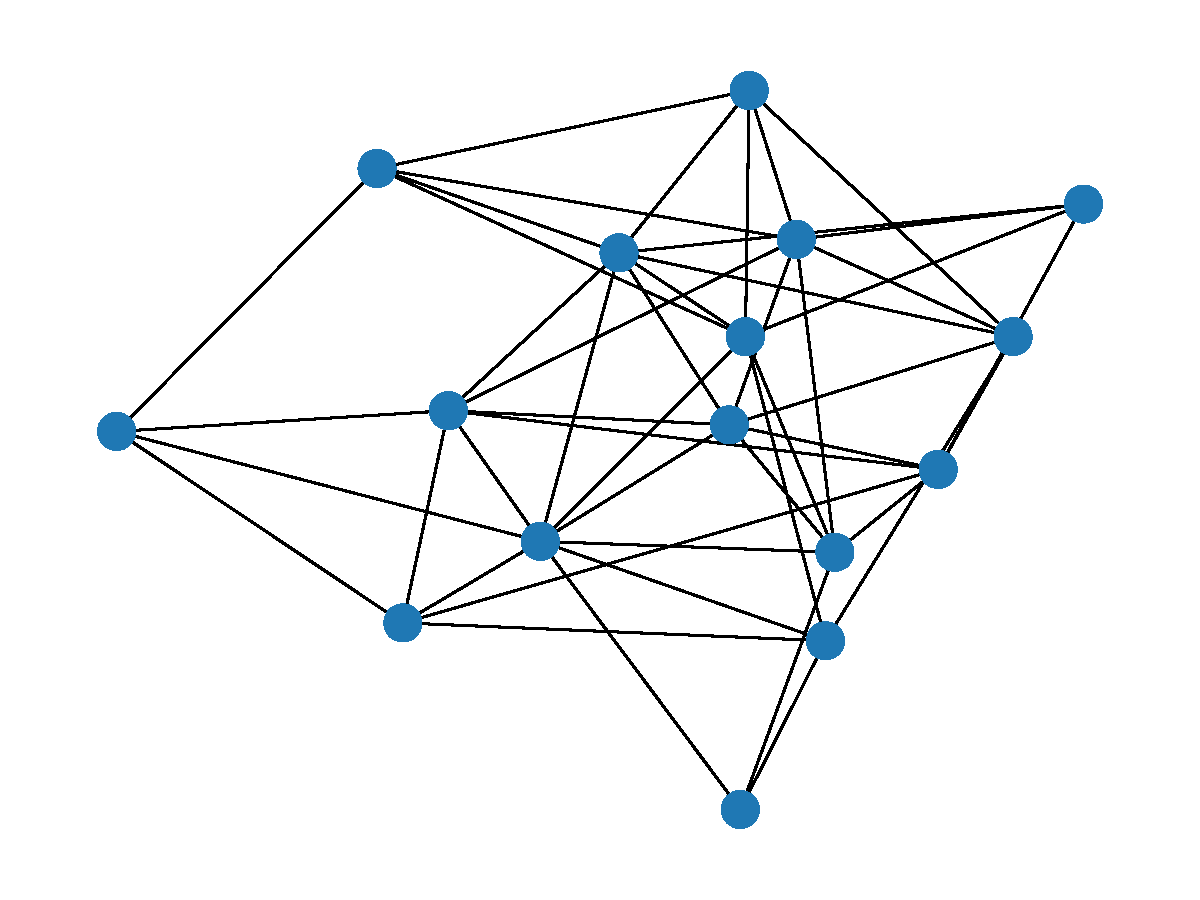
\includegraphics[width=0.4\textwidth]{./figures/results/er_graph_8_a_params.pdf}
  \caption[Example 8-\si{\angstrom}-graph vs Erd\"os-Rényi graph with the same
  number of nodes and edges.]{Example 8-\si{\angstrom}-graph vs Erd\"os-Rényi graph with the same
    number of nodes and edges. The protein entry used here to obtain the
    8-\si{\angstrom} graph is an uncharacterized protein with TrEMBL ID
    A0A6Q8PFQ6. We chose it because it was the shortest protein found in the
    human proteome as predicted by the AlphaFold2 model.}
  \label{fig:er_comparison_8a_graph}
\end{figure}

Furthermore, we found that the sensitivity of the \acrshort{mmd} to perturbation was
greatly influenced by the graph representation extracted from the protein.
Namely, for $\varepsilon$ graphs (which overall seemed more stable than $k$-NN
graphs), the higher $\varepsilon$, the lower the sensitivity to low levels of
perturbation (Figure \ref{fig:mmd_sensitivity_eps}).

We introduced in Section \ref{sec:descriptors} and shown in Section
\ref{sec:results_protein_descriptors} two \emph{novel} protein-specific descriptors for
used in \acrshort{mmd}, which are both extremely fast to compute (Table \ref{tab:runtimes})
and are able to detect perturbations with a surprising sensitivity (Figure
\ref{fig:protein_specific_descriptors}).

Furthermore, we found that the Weisfeiler-Lehman kernel, introduced in Section
\ref{sec:methods_kernels}, applied to \acrshort{mmd} was able to detect perturbations
unable to be detected by traditional graph descriptors such as point mutations,
which are relevant for the protein domain (Section
\ref{sec:results_graph_kernels}). However, as with the rest of the perturbations,
the Weisfeiler-Lehman kernel is not sensitive to lower regimes of perturbation
(see Figure \ref{fig:wlk}).
This can be alleviated by using an alternative descriptor such as the ESM
protein embedding introduced in Section \ref{sec:evalproblem}, which is more
sensitive to lower rates of point mutation (see Figure
\ref{fig:esm_descriptor}).

We analyzed the \acrshort{mmd} obtained from kernels operating on persistence diagrams in
Section \ref{sec:results_topo_kernels}, which also seemed very promising since
\acrshort{mmd} values leveraging topological kernels both exhibit high correlations to
point cloud perturbations and low inter-run variance.

\section{Practical Recommendations}\label{sec:discussion_recommendations}

Leveraging those key findings, we now formulate a set of recommendations for a
practitioner who needs to evaluate a generative protein model using one of the
protein representations highlighted above.


\subsection{Setup And Baselines}\label{sec:discussion_baselines}
% p-values, violin plots to visualize mmd.

Overall, we advise the practitioner to carefully evaluate certain baselines when
possible. The first would be to evaluate the \acrshort{mmd} between different
i.i.d. samples of the reference distribution to establish the range of
\acrshort{mmd} to be expected in the best case, which we refer to as the
\emph{positive control}. We conducted such positive control for various MMD
configurations in Appendix \ref{sec:mmd_baselines}. From there, an accurate
assessment of the quality of the model can be made. If the kernel and data
representation allows it, it is also advisable to establish a \emph{negative
control}. This would show the worst possible performance between any two
distributions. Typically, for the biased estimate of \acrshort{mmd}, this value
is $\sqrt{2}$. If this is not possible, as is the case in this thesis (e.g.
there is no negative control for all \acrshort{mmd} values perturbed using the
Gaussian noise), it is useful to examine cases of extreme perturbations and
compare the resulting \acrshort{mmd} values to those. Such an assessment can
provide a surrogate for the negative control and confers a sense of scale for
the particular problem tackled.

Moreover, since the \acrshort{mmd} statistic is the basis for a kernel two-sample test
\citep{gretton2012kernel} (see also Section \ref{sec:mmd}), one can easily
estimate a $p$-value from the statistic between the model's generated
distribution and the empirical distribution.

\subsection{Sensitivity Of MMD}\label{sec:discussion_right_mmd}
% Comment also on std dev - could potentially help with the p-value if high.
Depending on the stage of modeling and the coarseness of the desired samples,
one might choose different \acrshort{mmd} configurations. As we have shown in Figure
\ref{fig:mmd_sensitivity_eps} and discussed in Section
\ref{sec:results_sensitivity}, choosing a lower threshold $\varepsilon$ to
extract $\varepsilon$-graphs from a protein point cloud results in a higher
sensitivity to a host of perturbation. In practice, this means that the lower the
$\varepsilon$, the better the \acrshort{mmd} will be at discerning perturbed (i.e.
generated) samples from reference samples. This might be desirable if one needs
highly similar distributions of graphs. However, it can sometimes be desirable
to relax this requirement, e.g. to explore a larger part of the design landscape
or make a rougher assessment of the generated samples for debugging purposes.

In addition, when choosing an \acrshort{mmd} configuration, one should also investigate the
magnitude of inter-run variance, as it can also render a particular
configuration of \acrshort{mmd} useless since the possible ranges of \acrshort{mmd} values can be too
wide to make any assessment as to the quality of the generated samples

\subsection{Realistic Proteins}\label{sec:discussion_realistic_proteins}

Another setting in which some key findings of this study can be useful is in the
context of assessing \emph{realistic} proteins. Defining realistic proteins take on a
myriad of aspects: i.e. are the generated protein sequences realistic? In this
case, one might use a Weisfeiler-Lehman kernel or an ESM embedding to answer
this. The literature, however, suggests that using embeddings does not yield the
same kernel parameters depending on the perturbation applied to the sequence. As
such, it is recommended to use a spectrum kernel \citep{leslie2002spectrum} for
sequences (see \cite{kucera2022conditional}, Section 4.1). There are, however,
other aspects of proteins related to their resulting shape to check. For this
purpose, the protein-specific descriptors devised in this thesis and introduced in
Section \ref{sec:descriptors} whose results are shown in Section
\ref{sec:results_protein_descriptors}, Figure
\ref{fig:protein_specific_descriptors} can be used. This way, an unusual angle
or abnormal interatomic distance distribution observed in the data will be
reflected in the \acrshort{mmd} value.

\subsection{Kernels and Kernel Parameters}
% Kernel recommendations
In this thesis, we often observed that the linear kernel and RBF kernels with
$\sigma<1$ were often effective to detect perturbations, and $\sigma>1$
resulting in insensitive and unstable \acrshort{mmd} values. Investigating the mean
distance distribution between the various embeddings of data points (Appendix
\ref{sec:distance_dist}) we can see that this is probably because the order of
magnitude of the data descriptors is consistently higher than this threshold. We
discuss the rough order of magnitude of the data and its impact on the choice of
$\sigma$ in Appendix \ref{sec:distance_dist} as well.
% TODO: add supplementary plot

\section{Limitations And Future Directions}\label{sec:discussion_limitations}

Now that we summarized the main findings of this thesis (Section
\ref{sec:key_findings}) and formulated a set of recommendations to the
practitioner (Section \ref{sec:discussion_recommendations}), we now highlight
important limitations of this thesis.

% TODO: investigate mean reciprocal rank

\subsection{Negative Control}

In Section \ref{sec:discussion_baselines}, we highlighted the necessity of a
\emph{positive control}. While this is possible for certain kernels (e.g. for
the aforementioned spectrum kernel, see \cite{kucera2022conditional} for
details), many of the settings discussed in this thesis do not have such a
``negative control''. While one could use absolute \acrshort{mmd} values of perturbed sets
of proteins as a reference for subpar performance, it is still recommended to find
appropriate pathological cases for specific applications to estimate what a worse-case
\acrshort{mmd} value might take.

% Useful??
% \subsection{Expressive Power of Histograms}
% Discuss descriptors with bin_ranges not able to capture extreme cases

% \subsection{Neural Network Pathologies On Unseen Data}
% Extrapolation is the issue
% ESM might work unpredictably on unseen sequences
% Mention unbiased kernels such as the spectrum kernel

\subsection{TDA Limitations}\label{sec:tda_limitations}

One of the novel applications of \acrshort{tda} discussed in this thesis is its adoption in
\acrshort{mmd} by computing the kernel on two collections of point clouds, hence leveraging
the shape of the proteins in the calculations. Two challenges face this
approach. The first is computation time (see Table \ref{tab:runtimes} and
discussion in Section \ref{sec:results_runtime}): the Vietoris-Rips filtration
was expensive to compute. The second drawback is expressivity: the vanilla
version of the Vietoris-Rips filtration is not sensitive to amino acid changes.
Both issues could be tackled by dividing each point cloud into 20 different
points cloud (1 for each type of amino acid) following a similar approach as was
done for atoms, which has been shown to be powerful \cite{jiang2021topological}.
The benefits of this approach are two-fold. On the one hand, it makes the
Vietoris-Rips filtration sensitive to changes in the amino acids in addition to
shape-related changes. On the other hand, it
speeds up computation time, because each point cloud is more sparsely populated
(see Section \ref{sec:results_runtime} for details), and because
each amino acid-specific point cloud can be computed in parallel.

% \acrshort{tda} on different point clouds
% computational complexity

\subsection{Mode Collapse And Mode Drop}\label{sec:mode_collapse_mode_drop}

Mode collapse and mode dropping are the two distinctive and common failure modes
of generative models \citep{salimans2016improved}. We define mode collapse as
the situation when a particular type of generated output (i.e. intra-mode
outputs) lacks variety. Mode drop refers to the situation when some modes of the
data are not represented in the generated output. Both arise when implementing
common generative model architectures such as \acrshort{gans}. Although some
methods have been devised to tackle such issues for \acrshort{gans}
\citep{arjovsky2017wasserstein, goodfellow2014generative}, it remains a
challenge that needs to be tackled by suitable evaluation measures. Since
\acrshort{mmd} takes the average of kernel matrices (see Equation \ref{eq:mmd}),
we anticipate its potential to detect mode collapse is limited, since
\acrshort{mmd} is invariant to changes that do not affect the mean of the
distributions to be compared.

While others have simulated such pathologies in synthetic datasets by manually
changing the composition of each mode and investigating evaluation metrics'
behaviour to it \citep{thompson2022evaluation}, applying such mode-related
perturbations to protein datasets have yet to be tackled and are beyond the
scope of this thesis. One method that could be used to investigate such
situations would be to modify the composition of various protein families,
within which proteins share structural similarities. To simulate mode collapse,
one could impoverish the number of proteins within a given family. To simulate
mode drop, one could remove those proteins entirely from the distribution.
Defining protein families could be achieved by looking at evolutionary links
between proteins using for instance CATH database \citep{orengo1997cath}.
Alternatively, one could also use structural hierarchies to define protein
families using the SCOP database \citep{murzin1995scop}.

\subsection{Kernel Composition}

Kernel composition is a mechanism by which one can chain kernel functions to
combine different representations of data points by either multiplying or adding
kernel matrices. Although we did not investigate kernel composition here,
because we wanted to assess the expressive power of individual kernels and
representations, a practitioner could combine those to obtain an even richer
descriptors combining the advantages of various \acrshort{mmd} configurations in this
thesis.

\section{Summary}

% In this chapter, we (i) summarized the key findings of this thesis in order to
% (ii) make a set of recommendations for a practitioner. Finally, we (iii)
% detailed some of the limitations of and future work that could be done building
% on the findings presented in this thesis.

In Section \ref{sec:key_findings}, we show that the \acrshort{mmd} on the types of graphs used in this
thesis is more stable than for synthetic graphs used in the literature. We
highlight the sensitivity of \acrshort{mmd} to the underlying parameters used to extract
graph representations of proteins. We then discuss the behavior of the
protein-specific descriptors introduced in this thesis. Furthermore, we
summarize the findings related to the graph kernel investigated in this thesis.
Finally, we sum up the results on a set of known kernels and descriptor
functions used for \acrshort{mmd}.

In Section \ref{sec:discussion_recommendations}, we first advise the
practitioner to establish a positive control to establish a best-case \acrshort{mmd} value.
Secondly, if conditions allow, one can also establish a negative control to
estimate a worst-case \acrshort{mmd} value. We also redirect the practitioner to our
findings to use representations that are more or less susceptible to
perturbations depending on the required fidelity of generated samples to the
reference distribution. We then move on to discuss the various aspects that
constitute the assessment of what makes a realistic protein. We conclude our
recommendations with relevant kernel choices.

We discuss the limitations of this thesis in Section
\ref{sec:discussion_limitations} by starting off with discussing the often
unfeasible crafting of negative controls. We then move on to discussing the
limitations of a particular set of \acrshort{mmd} configurations using \acrshort{tda} and how to
potentially solve it. We then highlight the fact that \acrshort{mmd} is insensitive to
generative model pathologies that do not affect the mean of the distributions
due to the averaging of the kernel matrices. We close our discussion by
highlighting the composability of the kernels, which could greatly expand the
building blocks highlighted in this thesis in future work.
